\chapter{PHƯƠNG PHÁP ĐỀ XUẤT}\label{chap:proposedmethod}
\textit{Chương này chúng tôi trình bày giải pháp mà chúng tôi đề xuất để giải quyết bài toán phân đoạn gan và mạch máu trên ảnh chụp cắt lớp vi tính. Bao gồm mô hình, hàm mục tiêu, quá trình huấn luyện. }

\section{Định nghĩa bài toán}
\textbf{Tổng quan bài toán:} Sau quá trình nghiên cứu và tìm hiểu các hệ thống phân đoạn hình ảnh y khoa , chúng tôi xác định được bài toán cần giải quyết bao gồm 3 nhiệm vụ chính: \textit{Huấn luyện mô hình gắn nhãn cho bộ phận gan và mạch máu, phát triển công cụ làm nhãn được cung cấp bởi GVLab đồng thời tích hợp mô hình phân đoạn tự động vào hệ thống}.
\vspace{-0.25cm}
\begin{itemize}
    \item[] \textbf{Dữ liệu đầu vào}
    \item Bộ ảnh CT 3 chiều của 1 bệnh nhân bất kỳ.
    \item Nhãn phân đoạn cơ quan tương ứng của bộ ảnh CT đó.
    
    \item[] \textbf{Dữ liệu đầu ra}
    \item Kết quả phân đoạn gan và mạch máu từ khối ảnh CT ban đầu.
\end{itemize}
\vspace{-0.25cm}
Sau khi xác định thông tin đầu vào và kết quả đầu ra của bài toán, chúng tôi đề xuất phương án thiết kế hệ thống với những tham khảo từ các công trình liên quan được trình bày trong phần tiếp theo.

\section{Hướng tiếp cận đề xuất}
Mô hình Unet2D \cite{Unet} đã đạt được nhiều kết quả khả quan trong lĩnh vực phân đoạn tế bào. Tuy nhiên, do có sự khác nhau về tính chất của 2 tập dữ liệu: bài báo Unet tập dữ liệu chỉ bao gồm những hình ảnh 2 chiều về tế bào trong khi đó tập dữ liệu về gan (máu) lại chứa thêm thông tin của chiều thứ 3 (là tập hợp các lớp cắt liên tiếp nhau trên cơ thể). Do đó việc quan tâm đến các thông tin không gian trong 3 chiều của các đối tượng có thể đem lại nhiều kết quả khả quan cho bài toán này. Bên cạnh đó, đã có nhiều công trình sử dụng Unet3D \cite{unet3d} làm mô hình chính để thực hiện các cải tiến và đạt những mục tiêu nhất định. Bên cạnh đó, nhờ vào những nghiên cứu trước trong lĩnh vực phân tích ảnh y khoa (\cite{Deepsupervision}, \cite{LV_LIVER}, \cite{LV_VESEL}), một mô hình đã đạt được độ chính xác đáng được nhắc tới là mô hình Unet3D sử dụng phương pháp giám sát sâu để huấn luyện \cite{Deepsupervision}. Mô hình này đã đạt được độ chính xác 95\% trong quá trình phân đoạn gan được \cite{LV_LIVER} triển khai. Do đó đây sẽ là mô hình cơ sở để nhóm phân tích phát triển các mô hình mới cho bài toán phân đoạn này. 

Kiến trúc U2net3D* được nhóm đề xuất được dựa trên ý tưởng của mô hình $\mathrm{U}^2$net (được giới thiệu ở phần \ref{u2net_arch}) cùng với mô hình Unet3D sử dụng giám sát sâu (Deep supervision). Đầu tiên để đánh giá mức độ hoạt động của 2 mô hình liên quan nhóm đã dựng lại các thí nghiệm áp dụng cho gan và mạch máu đối với 2 mô hình này (chi tiết ở chương \ref{chapter:experience}). 

Đối với mô hình $\mathrm{U}^2$net, đây là mô hình phân đoạn cho bài toán phát hiện đối tượng nổi bật trong ảnh với kích thước đầu vào ở dạng 2 chiều. Tuy nhiên, đối với việc xử lý 2 chiều trên ảnh CT không đạt hiệu quả cao bởi việc mất thông tin không gian ở chiều thứ 3 (có thể thấy ở thí nghiệm \ref{exp:2dvs3d}) hiện tại mục tiêu hướng tới của chúng tôi là sử dụng được chiều thứ 3 của ảnh CT, do đó nhóm đã tiến hành chuyển đổi dựa trên mô hình $\mathrm{U}^2$net sử dụng cho ảnh 3 chiều. Tuy nhiên bởi do tính chất của kiến trúc mạng quá lớn, việc chuyển giao qua mô hình 3D không thể thực thi. Số lượng tham số huấn luyện tăng từ 20 triệu tham số lên đến 100 triệu tham số cùng với việc số lượng bản đồ đặc trưng 3D trong quá trình tính toán tăng đáng kể. Do đó mô hình 3D theo kiến trúc $\mathrm{U}^2$net được bài báo đề xuất không thể huấn luyện tại thời điểm này vì không đủ phần cứng. Vì vậy, nhóm sẽ kế thừa ý tưởng kiến trúc khối Residual U-Block để phát triển. Khối Residual U-Block (RSU) sẽ có kiến trúc như hình \ref{img:Block}.a .

\begin{figure}[H]
    \subfloat[Residual U-Block -- RSU-3(In, M, Out)]{
    	\begin{minipage}[c][1.5\width]{0.5\textwidth}
    	   \centering
    	   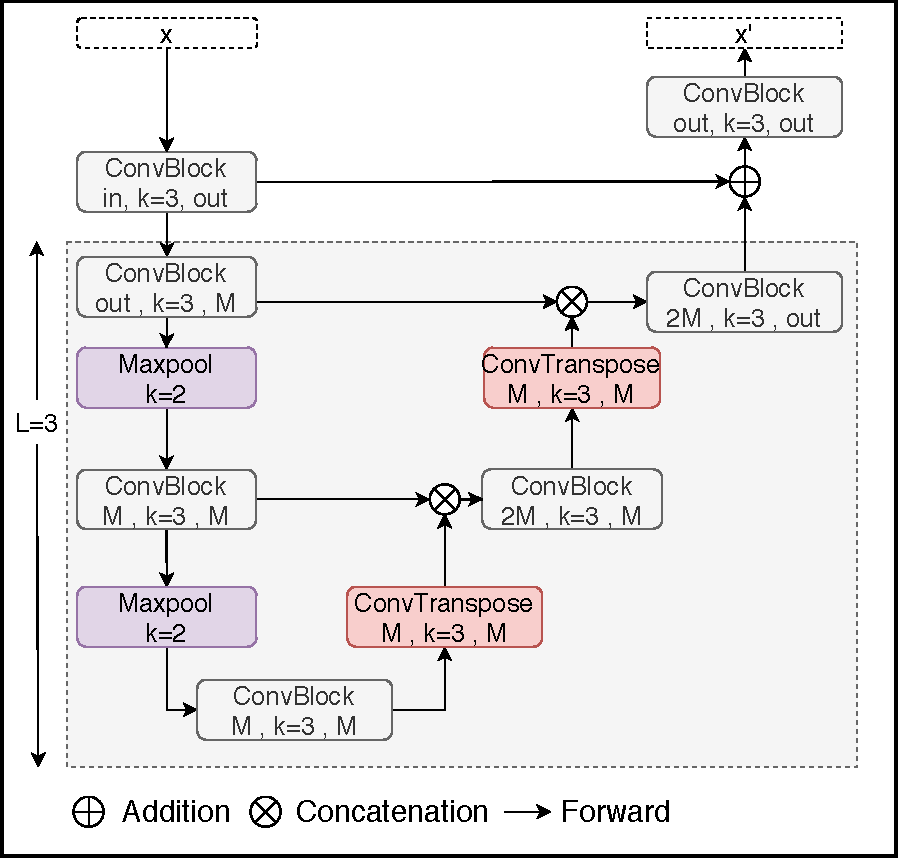
\includegraphics[width=1.35\textwidth]{images/blood/RSU_L3.pdf}
    	\end{minipage}}
	\hfill 	
    \subfloat[ConvBlock(In, M, Out)]{
    	\begin{minipage}[c][1.15\width]{0.65\textwidth}
    	   \centering
    	   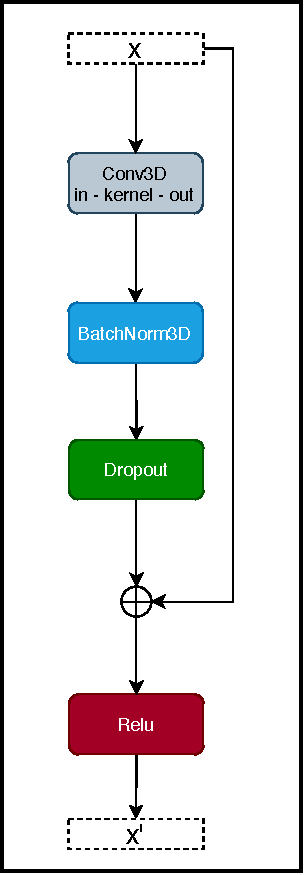
\includegraphics[width=0.4\textwidth]{images/blood/convblock.pdf}
    	\end{minipage}}
\caption{Kiến trúc các khối trong mô hình mạng}
\label{img:Block}
\end{figure}
\begin{itemize}
    \item Mỗi khối ConvBlock sẽ bao gồm các phép: Tích chập, Batchnorm, Dropout và hàm kích hoạt Relu. Bên cạnh đó khối có sử dụng phép kết nối tắt (residual) giúp hạn chế được tình trạng tiêu biến đạo hàm (vanishing gradient).
    \item Khối RSU sẽ bao gồm các siêu tham số: In, M, Out. Trong đó In là số kênh đầu vào của input, Out là số kênh đầu ra của các đặc trưng, M là số lượng các bản đồ đặc trưng được trích xuất trong các lớp trung gian. 
    \item[] Để lựa chọn các siêu tham số này một cách hợp lý, nhóm sẽ tiến hành các thí nghiệm trên các tham số khác nhau để kiểm chứng mô hình. 
\end{itemize}

\section{Kiến trúc mô hình phân đoạn đề xuất}\label{proposed-model}
Đầu tiên kế thừa sự thành công của mô hình CNN3D \cite{LV_LIVER} Nhóm đã chọn kiếm trúc này để làm mô hình cơ sở với ý tưởng tích hợp các khối RSU đại diện cho một kiến trúc Unet thu nhỏ vào mô hình CNN3D. Kiến trúc mô hình tổng quát dựa trên CNN3D như sau:
\begin{figure}[H]
    \centering
    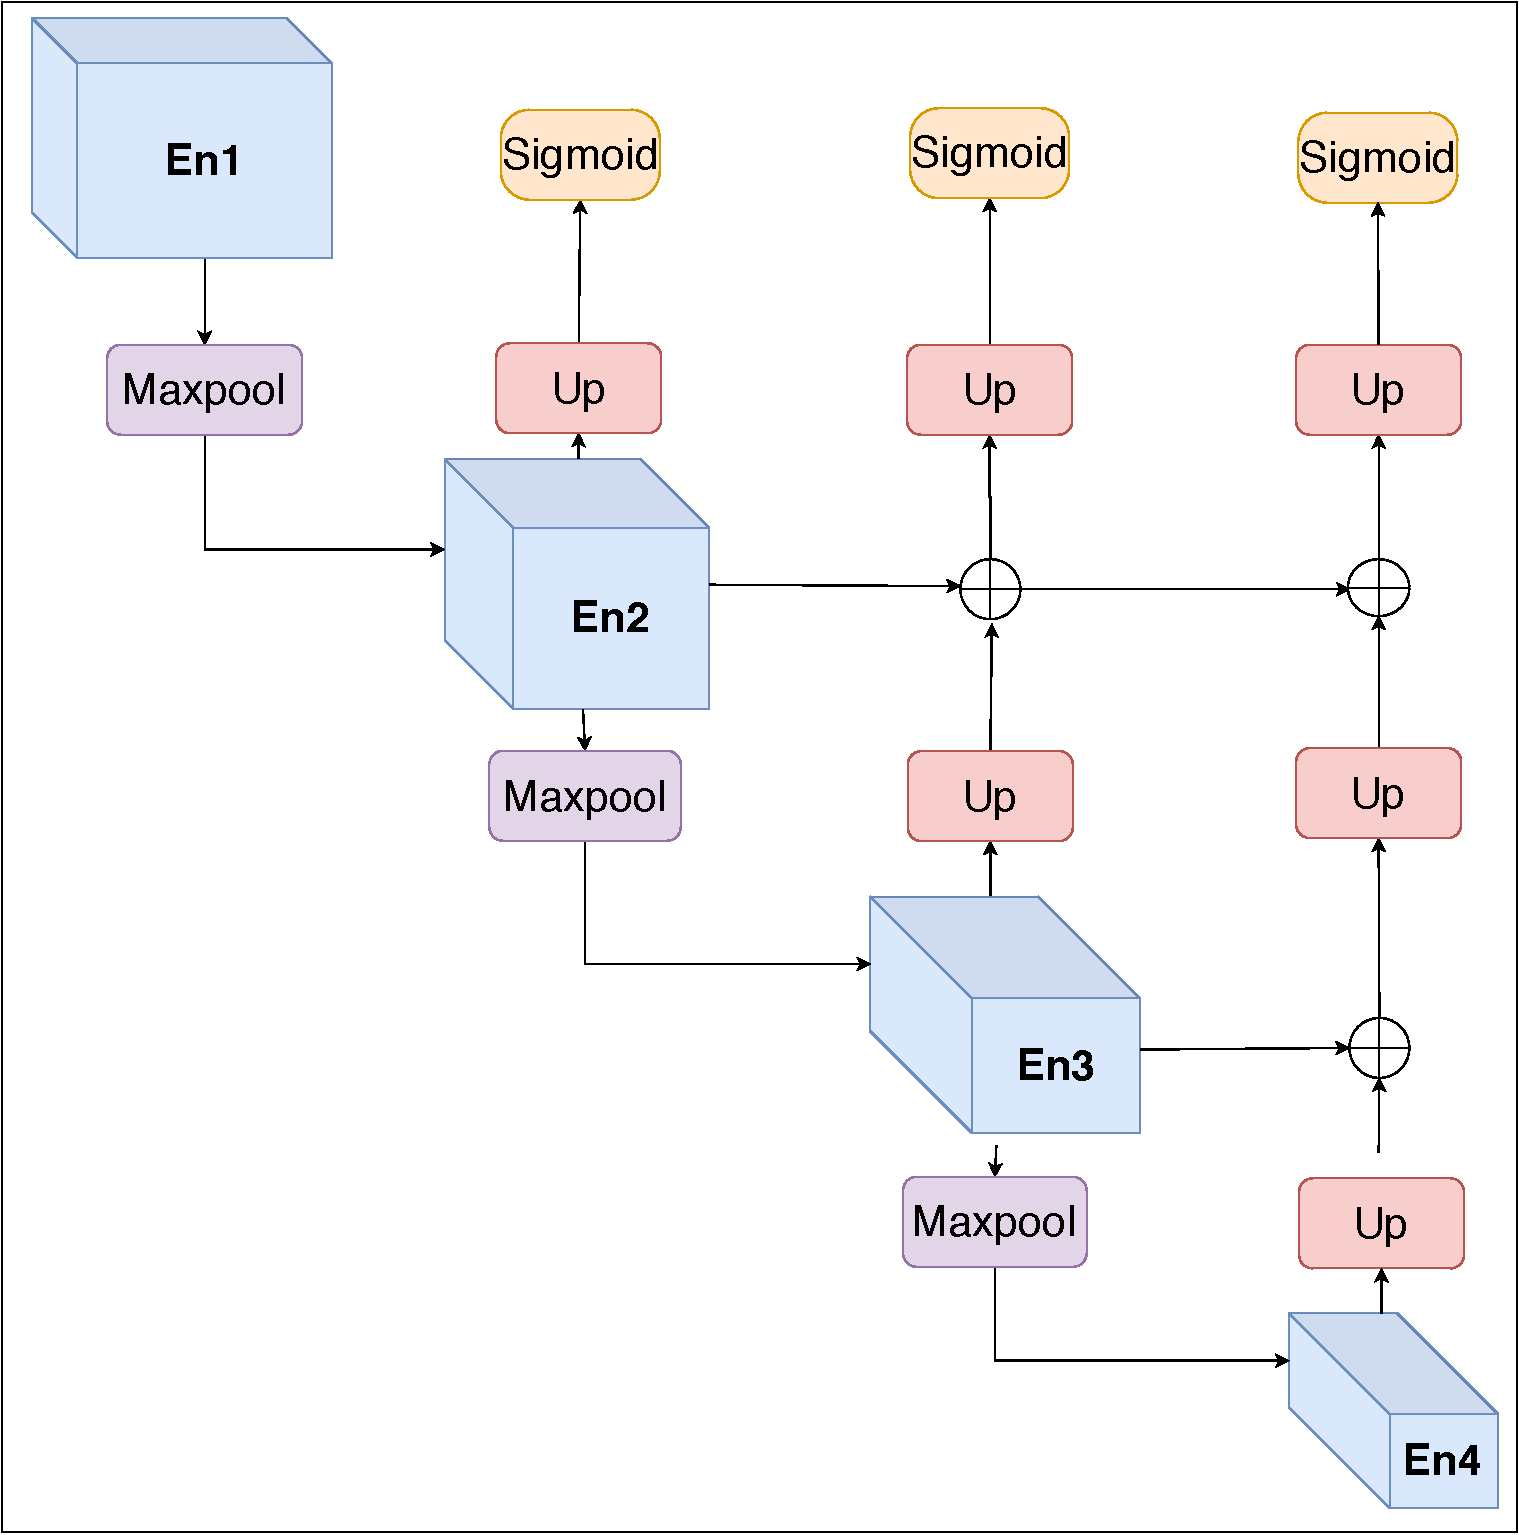
\includegraphics[scale=0.6]{images/blood/u2net3d-abstract.pdf}
    \caption{Kiến trúc mô hình tổng quát.}
    \label{fig:u2net3d-abstract}
\end{figure}

\newpage
\subsubsection{Khác biệt giữa kiến trúc mô hình đề xuất và mô hình CNN3D\cite{LV_LIVER}}
\begin{enumerate}
    \item Thay vì việc sử dụng các khối tích chập liên tiếp nhau trong quá trình mã hóa thông tin đầu vào, nhóm xin đề xuất việc thay những khối tích chập này thành những mô hình Unet thu nhỏ có tên là RSU.
    \item Ngoài ra, các phép kết nối tắt giữa các đặc trưng trích xuất trong bộ mã hóa sẽ được kết nối với đặc trưng từ bộ giải mã (có thể so sánh sự khác biệt này dựa trên hình \ref{fig:CNN3D} và Hình \ref{fig:u2net3d-abstract}). Nhờ vào các kết nối tắt này, các đặc trưng được sinh ra trong quá trình giải mã sẽ được kết hợp với thông tin ngữ cảnh trước đó giúp tăng độ chính xác của quá trình giải mã. Ngoài ra còn phần nào giúp được việc hạn chế quá trình tiêu biến đạo hàm.
\end{enumerate}
\vspace{-1cm}
\subsubsection{Bộ mã hóa}
\begin{enumerate}
    \item[] Bộ mã hóa của mô hình U2net3D* bao gồm 4 khối. 
    \item Khối En1 là khối tích chập thông thường bao gồm 2 khối ConvBlock (hình \ref{img:Block}.b)(mỗi khối bao gồm các phép tích chập, batchnorm, dropout, relu) liên tiếp nhau tại tầng thứ nhất. 
    \item Tại tầng thứ 2 trở đi sẽ là các khối RSU với số tầng của mỗi khối giảm 1 sau qua tầng tiếp theo. Khối RSU đầu tiên có số tầng là 3.  
    \item Thông qua các thí nghiệm chọn các siêu tham số cho mạng, chúng tôi nhận thấy việc sử dụng số lượng bản đồ đặc trưng đầu ra tăng gấp đôi sau mỗi tầng đạt được kết quả tốt nhất thay vì đặt tất cả các khối cùng một số lượng các đặc trưng trích xuất qua mỗi lớp.
\end{enumerate} 
\vspace{-1cm}
\subsubsection{Bộ giải mã}
\begin{enumerate}
    \item Các đặc trưng được sinh ra trong quá trình trích xuất thông tin của các khối RSU sẽ được giải mã tương ứng trên từng nhánh. Khi giải mã tới các tầng tương ứng, bộ giải mã sẽ sử dụng phép kết nối tắt dựa trên thông tin trước đó của từng tầng. Điều này giúp cho mô hình học tốt hơn bởi giá trị đầu vào sẽ được phân bố học dựa trên các luồng, các đặc trưng sinh ra tại mỗi tầng sẽ được giám sát song song với kết quả đầu ra cuối cùng.
    \item Các đặc trưng ở lớp cuối cùng của bộ giải mã sẽ đi qua lớp tích chập có bộ lọc 1x1x1 để thu giảm số kênh, sau đó qua lớp kích hoạt Sigmoid sẽ thu được giá trị xác xuất dự đoán của từng voxel.
\end{enumerate}

\begin{figure}[H]
    \centering
    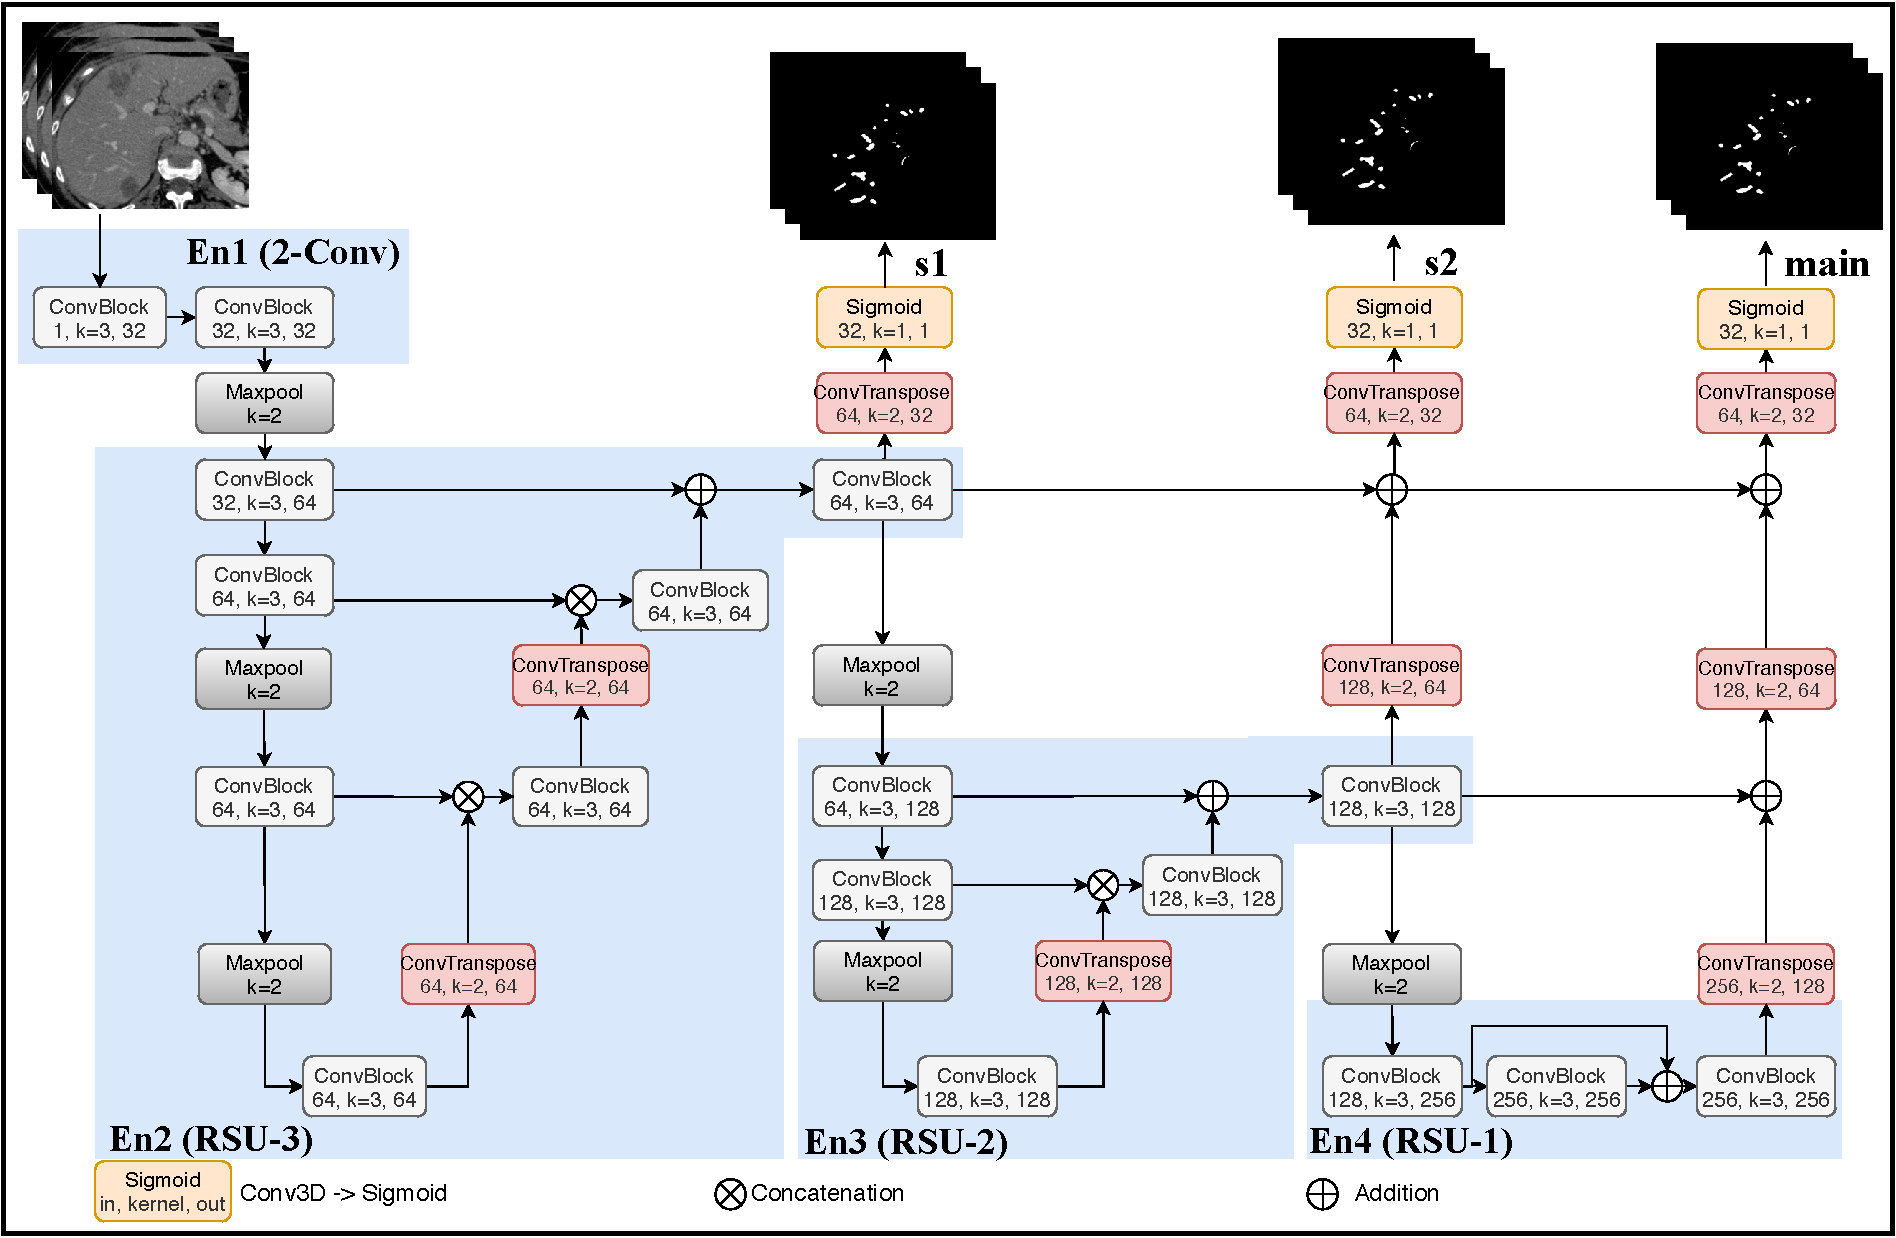
\includegraphics[angle=90,scale=0.6]{images/blood/u2net3d_arch.pdf}
    \caption{Kiến trúc mô hình chi tiết U2net3D*.}
    \label{fig:u2net3d-arch}
\end{figure}

\section{Hàm mục tiêu}
Trong bài toán học có giám sát (supervised learning), hàm mục tiêu (Objective Function) đóng vai trò quan trọng trong việc đưa ra giá trị phạt cho mô hình dự đoán sai bao nhiêu so với thực tế. Dựa vào đó, mô hình học cách cải thiện để đem lại kết quả tốt hơn sau mỗi lần học. Một số hàm mục tiêu được nhóm sử dụng để huấn luyện mô hình sẽ được trình bày bên đưới. Tất cả các hàm đều dùng cho bài toán phân đoạn nhị phân (2 lớp).

\subsubsection*{Binary Cross-Entropy Loss}
Hàm Binary Cross-Entropy (BCE) được dùng để đo lường tương quan giữa 2 phân phối xác suất dự đoán (q) và phân phối xác xuất thực tế (p).

\begin{align}
    \mathrm{L(q,p)} = -\sum_{i=1}^{C} \mathrm{p}_i \mathrm{log(q}_i)
\end{align}

Với $\sum_{i=1}^{C}\mathrm{p}_i = \sum_{i=1}^{C}\mathrm{q}_i = 1$ và C=2 đại diện cho 2 lớp cần dự đoán. Khi phân phối p và phân phối q càng tương quan thì giá trị của hàm BCE càng nhỏ, ngược lại khi hai phân phối này không tương quan giá trị hàm này sẽ càng lớn. Do đó, chúng ta đi tối ưu hàm Binary Cross Entropy cũng đồng nghĩa đi huấn luyện mô hình dự đoán phân phối q gần với phân phối p nhất. Đối với bài toán có 2 lớp giá trị nhãn $p_i$ sẽ nhận 2 giá trị 0 và 1. Do đó công thức trên có thể viết lại thành: 

\begin{align}
    \mathrm{L(q, p}) = -\log(\mathrm{q}) \\
    \nonumber
    \mathrm{q} = \begin{cases} 
              \mathrm{q} & \text{if } p = 1 \\
              1-\mathrm{q} & \text{otherwise}
          \end{cases}
\end{align}

Dựa vào đồ thị \ref{Focal-effective-weight} với gamma=0 (đây chính là đồ thị cho BCELoss) có thể thấy khi $\mathrm{q}$ tiến dần đến 1 thì hàm BCE tiến dần đến 0 - trường hợp mô hình tốt nhất tức là phân phối giữa p và q trùng nhau. Còn khi $\mathrm{q}$ tiến dần đến 0 thì hàm BCE tiến dần đến $\infty$ - mô hình tệ nhất. 

\subsubsection*{Focal Loss}
Đối với các bài toán bị mất cân bằng dữ liệu quan trọng, hàm BCE sẽ không hoạt động 1 cách hiệu quả. Ví dụ trong trường hợp bài toán phân đoạn ảnh, một bức ảnh có 100 pixel trong đó có 5 pixel là của nhãn A và số còn lại là của nhãn B. Một mô hình sẽ tiến hành phân loại và sử dụng hàm BCE để đánh giá cho từng pixel. Giá trị hàm loss sẽ là trung bình của tất cả giá trị BCE của 100 pixel này.  Như vậy, nếu mô hình chúng ta phân loại tốt lớp B nhưng không thể phân loại được lớp A điều này sẽ khiến cho hàm loss đem lại giá trị loss trung bình 100 pixel rất thấp vì 95 pixel đã được dự đoán đúng và chỉ 5 pixel thuộc lớp A dự đoán sai. Dễ nhận thấy đây là trường hợp tệ nhất mà chúng ta muốn tránh.

Do đó, với đề xuất của bộ phận nghiên cứu AI Facebook, họ đã đề xuất một sự cải tiến hàm Cross Entropy có trọng số được gọi là Focal Loss  (FL) được giới thiệu trong bài báo 'Focal Loss for Dense Object Detection' \cite{focal}. Với mục tiêu là cố gắng giảm sự đóng góp của các pixel vào trong giá trị loss tổng thay vì 100 pixel có mức độ ưu tiên như nhau ở ví dụ trên.

Với $\alpha$, $\gamma$ là các siêu tham số, giá trị $\alpha$ nằm giữa 0 và 1 để cân bằng tỉ lệ mẫu dương và mẫu âm. Giá trị $\alpha$ càng lớn thì độ đóng góp giá trị loss các mẫu dương sẽ càng cao hơn. Giá trị $\gamma > 0$ , có tác dụng làm giảm độ quan trọng của mẫu các mẫu phân loại đúng khi đóng góp vào giá trị của loss tổng. Như vậy $\gamma$ càng cao, hàm mục tiêu sẽ càng chú ý vào các mẫu bị phân loại sai, và giảm giá trị phạt cho các mẫu phân loại đúng. 

Công thức của hàm Focal Loss như sau:

\begin{align}
    \mathrm{FL(q, p)} &= -\alpha(1-\mathrm{q})^\gamma \log(\mathrm{q})\\
    \nonumber
    \alpha = \begin{cases} 
                    \alpha & \text{if } p = 1 \\
                    1-\alpha & \text{otherwise}
                \end{cases}
    &\quad and \quad
    \mathrm{q} = \begin{cases} 
              \mathrm{q} & \text{if } p = 1 \\
              1-\mathrm{q} & \text{otherwise}
          \end{cases}
\end{align}

Dựa vào đồ thị \ref{Focal-effective-weight} ta có thể thấy $\gamma$ càng lớn, kết hợp với các giá trị dự đoán đúng càng nhiều thì giá trị loss càng giảm mạnh. Như vậy nó sẽ góp phần đóng vai trò ít hơn trong hàm loss tổng. Chính nhờ vào điều này ta sẽ cân bằng được số lượng mẫu như ví dụ trên trong việc góp phần vào giá trị hàm mục tiêu.
\begin{figure}[H]
    \centering
    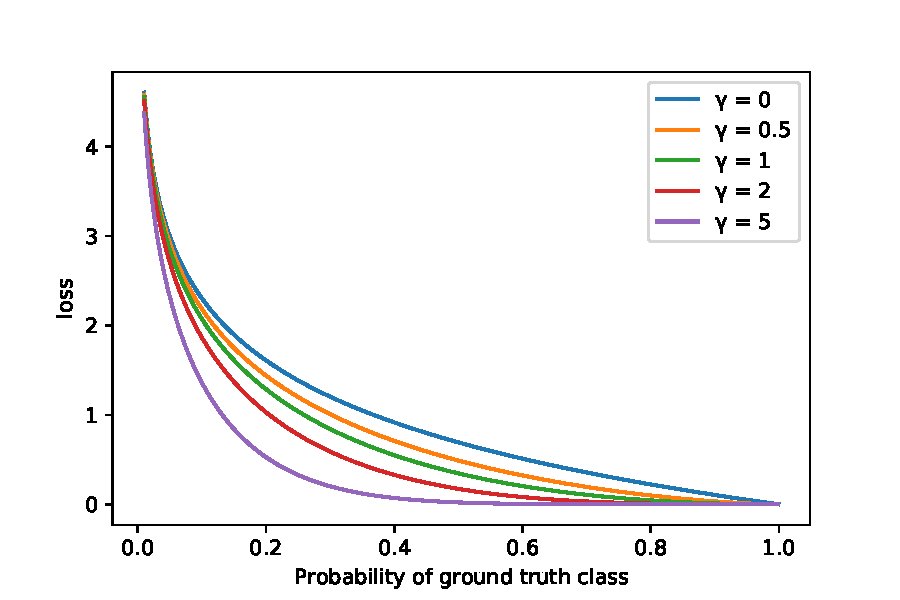
\includegraphics[width=10cm]{images/blood/focal.pdf}
    \caption{Sự ảnh hưởng của trọng số $\gamma$ đối với hàm focal loss $\mathrm{FL(q)=-(1-q)^\gamma \mathrm{log}(q)}$ }
    \label{Focal-effective-weight}
\end{figure}

\subsubsection*{Dice Loss}
Đây là hàm mất mát thường được sử dụng cho bài toán mất cân bằng giữa các lớp. Bằng cách lấy 1 trừ đi giá trị Dice, ta được công thức của Dice Loss:
\begin{align}
    L = 1 - 2\frac{\sum_{1}^{N}p_i*q_i}{\sum_{1}^{N}p_i + \sum_{1}^{N}q_i}
\end{align}
Trong đó, N là tổng số điểm ảnh. $p_i$ và $q_i$ lần lượt là giá trị nhãn và giá trị dự đoán của điểm ảnh thứ i, với $p_i \in \left \{ 0, 1 \right \}$ và $q_i \in \left [ 0, 1 \right ]$.

\section{Phương pháp huấn luyện}
\textbf{Phương pháp huấn luyện giám sát sâu}: Một số phần giải mã (decoder) thích hợp đã được thêm vào mạng để huấn luyện theo \textbf{phương pháp giám sát sâu}. Theo phương pháp này, hàm mất mát sẽ được tính từ hàm mất mát của tất cả các phần giải mã:
\begin{align}
    Loss = \mu_{1}Loss_{s1} + \mu_{2}Loss_{s2} + \mu_{3}Loss_{main}
    \label{LossU2net3D}
\end{align}

Mô hình sẽ có ba đầu ra, do đó hàm lỗi tổng sẽ có 3 thành phần tương ứng với từng đầu ra. Độ quan trọng của các đầu ra được xác định dựa trên giá trị của các siêu tham số $\mu_{1}$, $\mu_{2}$ và $\mu_{3}$. Hàm mất mát toàn phần lúc này là tổng hợp của hàm mất mát chính và các hàm mất mát phụ. Quá trình cập nhật tham số sẽ được chia sẻ giữa các luồng thay vì chỉ trên luồng chính. Cơ chế này giúp mô hình hội tụ nhanh hơn và có độ chính xác cao hơn. 

Hàm loss được sử dụng trong các thí nghiệm bao gồm 2 hàm BCELoss và Focal Loss (sử dụng độc lập với nhau) được sử dụng trong các thí nghiệm ở chương \ref{chapter:experience}.

Các siêu tham số sẽ được đặt tương ứng $\mu_1=1, \mu_2=2,  \mu_3=4$ với mục đích tăng dần độ quan trong trong quá trình giám sát việc trích xuất các đặc trưng theo từng tầng. Giá trị đầu ra của tầng cuối cùng sẽ chiếm phần quan trọng nhất và chính là kết quả cuối cùng của quá trình phân đoạn.
